\section{特征提取和分类} % <--- 这是本章唯一的 \section
\label{chap:feature_extraction}


\subsection{基于持续同调的特征构造方法}
\label{sec:tda_features}
% 核心:系统介绍将持久性图(PD)或其他PH输出转化为特征向量的方法。
在现代数据分析领域,面对日益增长的数据复杂性,例如三维点云数据和时间序列数据,开发能够捕捉数据内在结构和本质信息的特征构造方法至关重要。传统的特征提取方法往往侧重于数据的局部几何属性或统计特性,但在揭示高维数据的全局结构和拓扑形态方面能力有限。拓扑数据分析(Topological Data Analysis, TDA)作为近年来新兴的强大工具,特别是其核心方法——持续同调(Persistent Homology, PH),为从复杂数据集中提取鲁棒的拓扑特征提供了一个全新的视角\cite{gao2021newell}。

持续同调源于代数拓扑学,其核心思想是通过分析数据在不同尺度下的拓扑结构演化,来识别那些“持续”存在的、能够反映数据本质形态的特征,如连通分支(0维孔洞)、环状结构(1维孔洞)、空腔(2维孔洞)等 。与传统方法不同,持续同调能够捕捉数据的多尺度全局信息,并且对噪声和度量空间的微小扰动具有一定的稳定性。这些优点使得基于持续同调的特征在形状分类、分割、降噪、时间序列分析、点云理解、金融风险预测、生物医学以及材料科学等众多领域展现出巨大的应用潜力。

持续同调的计算结果通常被总结在持续图(Persistence Diagram, PD)中。持续图是一个信息丰富的多尺度描述符,它将数据中拓扑特征的“出生”(birth)和“死亡”(death)时间表示为二维平面上的一个多重点集。图上每个点 $(b_i, d_i)$ 对应一个拓扑特征,其横坐标 $b_i$ 是该特征出现的尺度,纵坐标 $d_i$ 是其消失的尺度,而 $d_i - b_i$ 则被称为该特征的“持久性”或“寿命”(persistence/lifetime)。

%插入图片

\begin{figure}[thbp!]
    \centering
    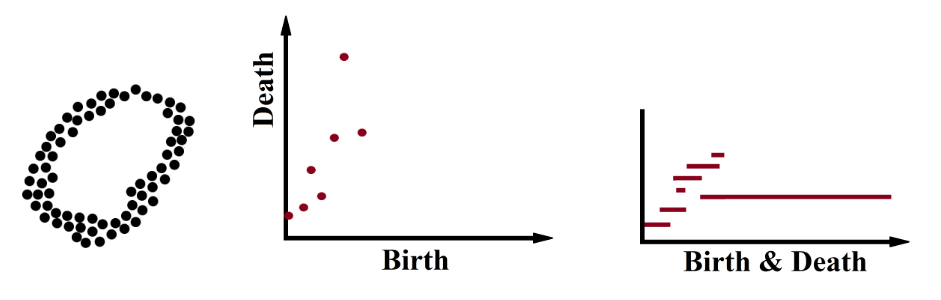
\includegraphics[width=1.0\textwidth]{figure/出生死亡示意图.png}
    \caption{持久性图和条形码}
    \label{fig:tde_example}
\end{figure}

然而,持续图本身作为一个数学对象(多重点集),其结构复杂且度量空间不完备,这使得它无法直接输入到标准的机器学习算法或深度学习框架中进行分析。因此,核心的挑战在于如何有效地量化和总结持续图中蕴含的拓扑信息,将其转化为具体的、可计算的、适用于下游任务的特征表示(Feature Representation)或描述符(Descriptor)。这正是持续同调特征构造方法研究的关键所在\cite{1021736289.nh}。

为了应对这一挑战,研究者们发展了多种策略来从持续图中提取特征。这些方法大致可以归纳为以下几类,也构成了本章将要深入探讨的主要内容。一种直接的方法是计算持久性图的统计描述符(Statistical Descriptors of PDs)。这类方法通过计算持续图上点的坐标(出生时间、死亡时间、持久性)的各种统计量来概括其分布特性。例如,可以计算不同维度同调群的特征总数、所有特征的总寿命或平均寿命、最长寿命(反映最显著特征)、显著特征(寿命超过某个阈值)的个数,以及基于寿命分布计算的熵值等。这些统计量提供了对持续图整体信息的宏观概括。

另一类方法侧重于基于贝蒂数(Betti Numbers)的表示。这类方法关注在不同尺度下拓扑特征的数量。贝蒂数 $\beta_k$ 直接量化了 $k$ 维孔洞的数量。通过追踪贝蒂数随尺度参数的变化,可以得到如贝蒂曲线(Betti Curves)等表示方法,它们反映了数据在不同尺度下的拓扑复杂度。

此外,还有一系列方法旨在将整个持续图的结构映射到一个更适合机器学习处理的空间,例如向量空间或函数空间。这些向量或函数空间嵌入方法中,有几种具有代表性。持续同调熵(Persistence Entropy, PE)是一种基于熵的标量描述符,形式简洁但可能信息损失较大(参考文献\cite{atienza2020stability})。持续性图像(Persistence Images, PI)通过对持续图上的点应用加权核函数(如高斯核)并进行积分,将其转化为稳定且维度固定的图像或向量表示(参考文献\cite{adams2017persistence} )。持续性景观(Persistence Landscapes, PL)将持续图上的每个点转换为一个“帐篷”函数,并取这些函数的 $k$ 次最大值,得到一系列分段线性函数,构成函数空间中的一个元素。

理解这些不同的特征构造方法的原理、计算方式、特性(如稳定性、可解释性、计算复杂度)及其优缺点,对于在具体应用中选择和设计合适的拓扑特征至关重要。本章旨在对上述几类基于持续同调的特征构造方法——即持久性图的统计描述符、基于贝蒂数的表示,以及具体的矢量化技术 PE、PI、PL 和 PC——进行详细的介绍和分析。通过对这些方法的阐述,我们将为读者构建一个关于如何从持续同调计算结果中提取有效特征的知识框架,为后续的理论研究和实际应用奠定基础。

\subsubsection{持久性图的统计描述符}
\label{sec:pd_stats}
% 原理:计算PD点的全局或维度相关的统计量。
% 示例:点的数量、寿命统计(总、均、最值、方差)、持久性熵、基于坐标/寿命的范数等。
% 文献:引用 Karan & Kaygun (2021) 中使用的熵和距离相关统计量。
% 优缺点:简单直观,但信息损失大,对噪声可能敏感。
在将持续同调应用于数据分析时,我们获得了信息丰富的持久性图(Persistence Diagram, PD)。然而,PD本身作为一个在$\mathbb{R}^2$空间中的多重点集 $\{(b_i, d_i)\}$,其结构不便于直接整合到许多标准的统计或机器学习框架中。为了克服这一障碍,研究者们提出了一系列方法来量化和总结PD中包含的拓扑信息,其中一类直接且直观的方法是计算PD的统计描述符。这些描述符旨在通过若干数值指标来捕捉PD的整体或关键特性,从而将抽象的拓扑结构信息转化为可操作的定量特征。

这类统计描述符通常直接利用PD中每个点 $(b_i, d_i)$ 的坐标信息,即拓扑特征的出生时间 $b_i$、死亡时间 $d_i$ 以及持久性(或寿命)$p_i = d_i - b_i$。通过对这些数值进行统计汇总,可以从不同侧面反映数据的拓扑结构。

一种基本的描述符是统计不同维度同调群(如$H_0, H_1, H_2$等)中检测到的拓扑特征的总数。这相当于计算PD中对应维度离对角线(即$d_i > b_i$)的点的数量。这个数量粗略地反映了数据在所考虑尺度范围内的拓扑复杂性。例如,在时间序列分析中,可以通过比较不同类别时间序列转化得到的点云所对应的PD中$H_1$(环状结构)特征的数量,来判断它们的结构差异。

除了特征的数量,特征的“寿命”或持久性 $p_i = d_i - b_i$ 是一个更关键的指标,因为它反映了拓扑特征的显著性——寿命长的特征通常对应于数据中更稳定、更本质的结构,而寿命短(即靠近对角线的点)的特征则可能与噪声或细微结构有关。因此,一系列基于持久性的统计量被提出。例如,可以计算某个维度下所有特征的总寿命($\sum p_i$),它反映了该维度拓扑特征的总体“能量”或显著性。将总寿命除以特征数量,则得到平均持久性(或平均寿命),它衡量了该维度特征的平均稳定性。研究发现,不同类别的数据在这些指标上可能呈现出显著差异,例如某一类时间序列可能普遍具有更长的平均$H_1$寿命。

在所有特征中,具有最大持久性的特征通常被认为是最重要的拓扑不变量。因此,最大持久性($\max p_i$)本身就是一个重要的统计描述符。它标识了数据中最“顽强”的拓扑结构。基于最大持久性,还可以定义“显著特征”的数量,即统计那些寿命超过某个阈值的特征个数,例如,可以取最大持久性的某个比例(如0.5倍)作为阈值。这种方法有助于过滤掉可能由噪声产生的短寿命特征,更聚焦于数据的核心结构。



此外,还可以考虑其他的统计量,例如寿命的方差、标准差、偏度或峰度,以更细致地刻画寿命分布的形态。或者,也可以考察拓扑特征之间的时间关系,例如计算在不同尺度下平均同时存在的同调群个数,这间接反映了特征在时间(尺度)维度上的重叠程度和复杂性,下面介绍一下论文中具体的使用方法:

Mittal的论文\cite{mittal2017topological}从动态系统时间序列数据经持久同调分析后得到的 $k$-维持久性图(其可表示为点集 $\Delta_k = \{(u_j, v_j)\}_j$,其中 $u_j$ 和 $v_j$ 分别为第 $j$ 个 $k$-维拓扑洞的诞生和消亡尺度)中,该研究提出了一系列拓扑特征以进行系统状态的量化。首先,定义第 $j$ 个 $k$-维洞的生命周期 $L_j$ 为:
\begin{equation}
    L_j = v_j - u_j
\end{equation}
基于各个洞的生命周期,可以确定该维度下所有洞的最大生命周期 $ML_k$:
\begin{equation}
    ML_k = \max_{j} \{L_j\}
\end{equation}
“相关 $k$-维洞的数量” $nrel_k$ 随之被定义为那些生命周期 $L_j$ 满足条件 $L_j > \theta \cdot ML_k$ 的洞的个数,其中 $\theta \in (0,1)$ 是一个预设比例。同时,“$k$-维洞的平均生命周期” $avg_k$ 计算如下,其中 $|\Delta_k|$ 为 $k$-维洞的总数:
\begin{equation}
    avg_k = \frac{1}{|\Delta_k|} \sum_{j=1}^{|\Delta_k|} L_j
\end{equation}
针对周期性行为,特别是在倍周期分岔现象中,“期望轨道周期” $K_{orbit}$ 通过以下方式估计:
\begin{equation}
    K_{orbit} = \left\lfloor \frac{S_1}{S} \right\rfloor
\end{equation}
这里,$S$ 是当前系统状态下对应单纯复形中的单纯形总数,$S_1$ 是一个已知的周期为1的基准稳定状态下的单纯形总数,而 $\lfloor \cdot \rfloor$ 表示向下取整函数。几何方面的特征也得到关注。对于一个由 $N_i$ 个 $M$-维顶点 $\{x_p = (x_p^{(1)}, \ldots, x_p^{(M)})\}_{p=1}^{N_i}$ 构成的特定 $k$-维洞 $i$,其“洞的直径” $D_i$ 定义为:
\begin{equation}
    D_i = \max_{1 \le p, q \le N_i} \{ d(x_p, x_q) \}
\end{equation}
其中 $d(x_p, x_q) = \|x_p - x_q\|_2$ 是顶点间的欧氏距离。由此,可以得到 “$k$-维洞的最大直径” $maxD_k$:
\begin{equation}
    maxD_k = \max_{i} \{D_i\}
\end{equation}
此外,为了量化不同洞之间的空间关系,首先计算每个洞 $i$ 的几何中心 $xc_i \in \mathbb{R}^M$。其第 $m$ 个坐标分量 $xc_i^{(m)}$ 计算方式为:
\begin{equation}
    xc_i^{(m)} = \frac{1}{N_i} \sum_{p=1}^{N_i} x_p^{(m)}
\end{equation}
任意两个 $k$-维洞 $i$ 和 $l$ 之间的距离则定义为其几何中心之间的欧氏距离:
\begin{equation}
    dist_k^{il} = \|xc_i - xc_l\|_2
\end{equation}
最终,“$k$-维洞之间的最大距离” $maxDist_k$ 被定义为所有不同洞对($i \neq l$)之间距离的最大值:
\begin{equation}
    maxDist_k = \max_{i \neq l} \{dist_k^{il}\}
\end{equation}
这些拓扑特征共同构成了对系统状态进行多维度拓扑量化描述的基础。

总而言之,持久性图的统计描述符提供了一套相对简单且直观的方法,用于从PD中提取定量的拓扑信息。通过计算特征数量、寿命的总和、平均值、最大值、显著性计数以及熵等指标,可以从宏观层面捕捉数据的拓扑结构特征。这些描述符易于计算和解释,并且已被证明在某些应用中能够有效地揭示不同类别数据之间的结构差异。然而,需要认识到,这些单一或少量的统计数值必然会损失PD中包含的大量几何和结构细节。相比之下,后续章节将要介绍的基于贝蒂数的表示方法以及向量/函数空间嵌入方法(如PI, PL, PC等)则试图以更全面的方式保留PD的结构信息,尽管这通常伴随着更高的计算复杂度和解释难度。理解这些统计描述符的含义和局限性,是选择合适拓扑特征进行数据分析的第一步。

\subsubsection{基于Betti数的表示}
\label{sec:betti_features}
% 原理:将Betti数视为滤过参数的函数或其离散采样。
% 文献:引用 Umeda (2017) 的Betti序列及应用;提及 Chung et al. (2020) 将其视为持久性曲线特例。
% 优缺点:反映特征数量变化,但损失位置信息。
继上一节探讨了通过计算持久性图(PD)的各类统计量来概括其拓扑信息之后,本节将介绍另一类重要的特征表示方法,它们直接关注于拓扑不变量的核心——贝蒂数(Betti Numbers)及其在持续同调框架下的演化。贝蒂数是拓扑学中的基本概念,第 $k$ 阶贝蒂数 $\beta_k$ 直观地量化了一个拓扑空间中 $k$ 维“孔洞”的数量。具体而言,$\beta_0$ 代表空间中连通分支的数量,$\beta_1$ 代表独立环路(一维孔洞)的数量,$\beta_2$ 则代表空腔或空洞(二维孔洞)的数量,以此类推。在代数上,$\beta_k$ 定义为第 $k$ 阶同调群 $H_k(K)$ 的秩(rank)。

然而,在持续同调的语境下,我们分析的不是单个静态的拓扑空间,而是一个通过尺度参数(例如,在VR复形构造中的邻域半径 $\epsilon$)索引的嵌套复形序列,即“过滤”(Filtration),记作 $\{K_t\}_{t \ge 0}$,其中 $K_s \subseteq K_t$ 当 $s \le t$。因此,仅仅计算某个特定尺度 $t$ 下的瞬时贝蒂数 $\beta_k(K_t)$ 无法完全捕捉到拓扑特征随尺度变化的持续性信息。持续同调的核心正是追踪这些特征(孔洞)的“出生”和“死亡”过程。与此相关的是持续贝蒂数(Persistent Betti numbers)的概念,它统计了在尺度区间 $[i, j)$ 内持续存在的 $k$ 维特征的数量,这与持续同调群 $H_k^{i, j-i}$ 的秩有关 (概念参考)。

尽管如此,考察瞬时贝蒂数 $\beta_k(K_t)$ 如何随尺度参数 $t$ 变化,本身就提供了一种有价值的拓扑描述方式。这种描述方式的核心是构建所谓的贝蒂曲线(Betti Curve)或贝蒂序列(Betti Sequence,当尺度参数离散时)。第 $k$ 阶贝蒂曲线是一个函数 $B_k: \mathbb{R}_{\ge 0} \rightarrow \mathbb{N}_0$,其在尺度 $t$ 处的值 $B_k(t)$ 就是复形 $K_t$ 的第 $k$ 阶贝蒂数,即 $B_k(t) = \beta_k(K_t)$ (相关概念见于 )。这条曲线描绘了 $k$ 维孔洞的数量在过滤过程中的动态变化情况。

贝蒂曲线可以从持续同调的计算结果(如持久性条形码或持久性图)中导出。对于一个给定的尺度 $t$, $B_k(t)$ 的值等于在 $k$ 维持久性条形码中,那些生命周期区间 $[b_i, d_i)$ 包含 $t$(即满足 $b_i \le t < d_i$)的条带的数量。换言之,它统计了在尺度 $t$ 时“存活”的 $k$ 维拓扑特征的总数。

从贝蒂曲线 $B_k(t)$ 的形态中可以解读出数据的拓扑演化信息。曲线的峰值对应于 $k$ 维孔洞数量达到极大的尺度范围,反映了该维度拓扑结构最为丰富的阶段。曲线的上升段表示新特征的诞生速度超过了旧特征的消亡速度,而下降段则反之。曲线积分 $\int B_k(t) dt$ 与对应维度下所有特征的总寿命(即上一节讨论的总持久性)密切相关。因此,贝蒂曲线的整体形状可以作为一种概括性的拓扑指纹。

在实际应用中,贝蒂曲线本身(或其离散采样版本——贝蒂序列)可以直接用作特征向量。例如,可以将曲线在预定的一系列尺度值上进行采样,得到一个固定长度的向量,然后输入到机器学习分类器中。已有研究利用贝蒂序列作为特征成功应用于时间序列分类等任务 。相较于上一节的单一统计描述符,贝蒂曲线保留了拓扑特征数量随尺度变化的动态信息,提供了更丰富的描述。但相较于后面将要介绍的持续性图像或景观等方法,它仍然丢失了特征之间的配对信息(即哪个出生事件对应哪个死亡事件),仅仅追踪了总数的变化。这意味着不同的持久性图可能对应相同的贝蒂曲线。

总结来说,基于贝蒂数的表示方法,特别是贝蒂曲线和序列,提供了一种连接经典拓扑不变量和持续同调的桥梁。它们通过关注拓扑特征数量随尺度的演化,为数据提供了一种中等粒度的拓扑描述符,兼具一定的解释性和信息量。理解贝蒂曲线的构建和解读,有助于我们从“计数”的角度把握数据的多尺度拓扑结构。接下来,我们将进一步探讨那些旨在更全面捕捉持久性图几何结构或提供不同类型数值总结的特征构造方法,如持续同调熵、持续性图像、持续性景观和持久性中心。

\subsubsection{基于函数或映射的向量化方法}
\label{sec:pd_vectorization_mapping}
% 将PD映射为函数、图像或低维向量。

% 注意:下一级的具体方法 PL, PI, PC, P-Center 维持为 \subsubsection 内部的普通段落或列表可能更好,
% 避免层级过深。或者如果你确实需要区分,可以继续用 \subsubsection,但我这里暂时用 \paragraph 示意。
前述的统计描述符和基于贝蒂数的表示为持久性图(PD)提供了有价值的定量总结,但它们通常以牺牲大量细节信息为代价。为了更全面地捕捉PD中蕴含的丰富几何与拓扑结构,并生成更适合现代机器学习技术的输入,研究者们开发了一系列基于特定函数或映射的向量化方法。这些方法的核心思想是将PD这个多重点集整体地、结构化地映射到一个向量空间(如 $\mathbb{R}^n$)或函数空间(如 $L^p$ 空间)中。其目标通常是生成稳定(即对输入数据的微小扰动不敏感)、信息丰富且计算上可行的特征表示。本节将分别介绍几种主流的此类方法:持续同调熵(PE)、持续性景观(PL)、持续性图像(PI)和持久性中心(PC)。

\paragraph{持久性熵 (Persistence Entropy)}
\label{sec:feat_pe}
% 原理、文献、优缺点...
在众多向量化方法中,持续同调熵(PE)\cite{atienza2020stability}可以被视为一种基于特定函数(信息熵函数)的极简总结方式。它并非生成高维向量,而是将持久性条形码或等价的PD信息压缩成一个单一的标量值。其计算依据是持久性条形码 $B = \{[b_i, d_i)\}_{i=1}^n$ 中每个条带的长度(寿命)$l_i = d_i - b_i$。借鉴香农熵的定义,持续同调熵被定义为 $PE(B) = -\sum_{i=1}^{n} \frac{l_i}{L} \log(\frac{l_i}{L})$,其中 $L = \sum_{i=1}^{n} l_i$ 是所有条带的总长度。这个值衡量了条带寿命分布的复杂性或不确定性。PE的优点在于其计算极其简单快速,得到的结果是一个易于使用的单一数值特征。然而,其最大的缺点是信息损失巨大,它完全忽略了特征的出生和死亡时间信息,仅考虑了寿命的分布,因此可能无法区分具有不同结构但寿命分布相似的PD。正如一些研究指出的,单一的PE数值在直接应用时可能过于片面。尽管如此,在某些特定场景下或作为辅助特征,PE仍有其应用价值。

\paragraph{持久性景观 (Persistence Landscapes, PL)}
\label{sec:feat_pl}
% 原理、特点、文献、优缺点...
持久性景观 (Persistence Landscapes) \cite{1} 是一种将持久性同调信息转化为函数空间元素的拓扑数据分析工具,因其向量空间特性而易于同统计学与机器学习方法相结合。其构建始于持久性模块 $M$,从中定义Betti数
\begin{equation}
    \label{eq:betti_number} % 您可以为公式添加标签以便交叉引用
    \beta^{a,b} = \text{dim}(\text{im}(M(a \le b): M_a \rightarrow M_b))
\end{equation}
用以量化在尺度 $a$ 到 $b$ 间持续存在的拓扑特征数量。进一步,持久性景观被定义为一系列函数 $\lambda_k: \mathbb{R} \rightarrow \overline{\mathbb{R}}$,其中
\begin{equation}
    \label{eq:lambda_k_definition}
    \lambda_k(t) = \text{sup}\{m \ge 0 \mid \beta^{t-m,t+m} \ge k\}
\end{equation}
这里 $\lambda_k(t)$ 直观表示在参数 $t$ 附近至少有 $k$ 个拓扑特征持续存在的最大“寿命半径” $m$。这些景观函数具有非负性 ($\lambda_k(t) \ge 0$)、对于固定的 $t$ 关于 $k$ 的单调递减性 ($\lambda_k(t) \ge \lambda_{k+1}(t)$) 以及1-Lipschitz连续性 ($|\lambda_k(t) - \lambda_k(s)| \le |t-s|$)。若给定一个由点集 $D = \{(b_i, d_i)\}_{i=1}^N$ 构成的持久性图,其中 $(b_i,d_i)$ 为第 $i$ 个特征的生灭时间对,则相应的景观函数 $\lambda_k(t)$ 可计算为所有
\begin{equation}
    \label{eq:lambda_k_from_diagram_core}
    \max(0, \min(t-b_i, d_i-t))
\end{equation}
值中的第 $k$ 大值。这种将拓扑特征转化为函数的方法,使得对拓扑数据进行平均、定义范数和距离以及应用统计推断成为可能,为复杂数据分析提供了有力支持。

\begin{figure}[thbp!]
    \centering
    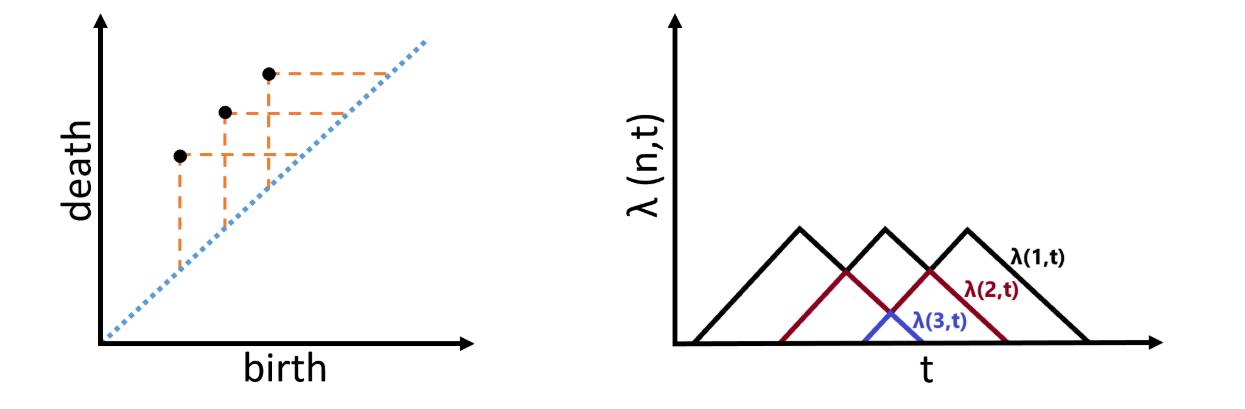
\includegraphics[width=1.0\textwidth]{figure/持久性景观.png}
    \caption{持久性图转化为持久性景观}
\end{figure}


\paragraph{持久性图像 (Persistence Images, PI)}
\label{sec:feat_pi}
持续性图像(PI)\cite{pun2022persistent}是当前应用最广泛的PD向量化方法之一,旨在生成稳定且易于被机器学习算法使用的固定维度向量表示 ,在多篇文献中均有提及或应用。PI的生成过程大致如下:首先,将PD中的点 $(b, d)$ 变换到“出生-持久性”坐标系,得到点 $(b, p)$,其中 $p = d-b$。接着,在每个变换后的点 $(b_i, p_i)$ 处放置一个二维概率密度函数(核函数),通常选用均值为 $(b_i, p_i)$、方差为 $\sigma^2$ 的高斯核 $\phi_{(b_i, p_i)}(x, y)$。为了强调持久性长的特征或根据需要调整不同区域的重要性,可以对每个核函数施加一个非负的权重函数 $f(b_i, p_i)$,该权重函数通常依赖于持久性 $p_i$。然后,将所有加权的核函数叠加起来,形成一个定义在 $\mathbb{R}^2$ 上的连续表面(或函数)$\rho_{B}(z) = \sum_i f(b_i, p_i) \phi_{(b_i, p_i)}(z)$。最后,在预先定义的二维网格上,对这个表面函数 $\rho_B$ 在每个像素(网格单元)$P$ 内进行积分 $\iint_P \rho_B(z) dz$,得到的积分值构成了该像素的灰度值。所有像素的值排列起来就形成了一个矩阵(图像)或一个向量(将矩阵展平)。PI的主要优势在于其表示的稳定性、生成结果的维度固定且属于欧氏空间,以及参数的灵活性(可以选择核函数、方差 $\sigma$、网格分辨率、权重函数等进行调整)。它也便于融合不同同调维度的信息,只需将各维度生成的PI向量拼接即可。但其缺点是结果可能受到参数选择的影响,并且如果PD中的点相对于网格分辨率来说过于稀疏,生成的PI向量可能包含大量零值。

\paragraph{持久性曲线 (Persistence Curves, PC)}
\label{sec:feat_pc}
% 原理、文献、优缺点...
持久性曲线(PC)\cite{chung2020persistent}是一种相对较新的PD向量化方法,旨在通过将PD映射到一个函数空间中来捕捉其几何结构 。其定义过程首先考虑一个持久性图表 $D$。设 $x, y, z \in \mathbb{R}$ 为实数。我们引入一个实值函数 $\psi(D, x, y, z)$,该函数的一个重要性质是当其第二和第三个参数相等时,函数值为零,即 $\psi(D, x, x, z) = 0$。此外,还需要一个统计量 $T$,它是一个作用于多重集 (multi-set) 的函数。基于这些组成部分,一条持久性曲线 $P(D, \psi, T)(x)$ 在点 $x$ 的值被定义为统计量 $T$ 应用于一个特定集合的结果,这个集合由所有满足 $b \le x < d$ 的持久性图表中的点 $(b,d)$ 经过函数 $\psi$ 转换后形成:
\begin{equation}
    P(D, \psi, T)(x) = T \left( \{ \psi(D, b, d, x) | (b,d) \in D, b \le x < d \} \right)
\end{equation}
其中,集合 $\{ (b,d) \in D | b \le x < d \}$ 通常被称为在 $x$ 处的基础盒 (fundamental box)。函数 $\psi$ 的选择至关重要,因为它决定了如何从持久性图表的每个点中提取信息。一个具体的持久性曲线实例是稳定生命周期曲线 (stabilized life curve)。为了定义它,首先定义点 $(x,y)$ 的生命周期为 $l(x,y) = y-x$。然后,对于稳定生命周期曲线,函数 $\psi$ 被特定化为标准化的生命周期:
\begin{equation}
    \psi_{\text{sl}}(D, b, d, x) = \frac{l(b,d)}{\sum_{(b',d') \in D} l(b',d')}
\end{equation}
其中分母是对图表 $D$ 中所有点的生命周期进行求和。若此时选择统计量 $T$ 为求和统计量,记作 $\Sigma$,则稳定生命周期曲线 $sl$ 可以表示为:
\begin{equation}
    sl(D)(x) = P(D, \psi_{\text{sl}}, \Sigma)(x) = \sum_{\substack{(b,d) \in D \\ b \le x < d}} \frac{y-x}{\sum_{(b',d') \in D} (d'-b')}
\end{equation}
通过这种方式,持久性曲线能够将复杂的持久性图表信息转换为一维函数(或其离散化后的向量),更便于后续的分析和机器学习应用。
\begin{figure}[htbp] % [htbp] 是图片位置浮动的建议参数
    \centering % 使图片在其容器内水平居中

    % 第一个图
    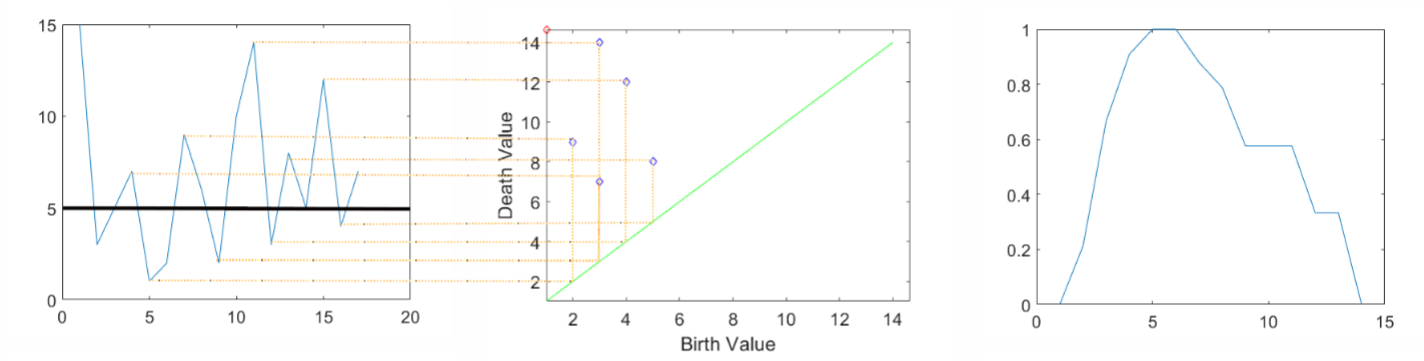
\includegraphics[width=1\textwidth]{figure/持久性曲线1.png} % 请替换为您的第一个图片路径和文件名
    % 您可以在两个图片之间添加一些垂直间距(可选)
    % \vspace{5mm} % 例如,增加5毫米的垂直间距
    % 或者简单地用一个空行来确保它们在不同行(通常默认就是如此)

    % 第二个图
    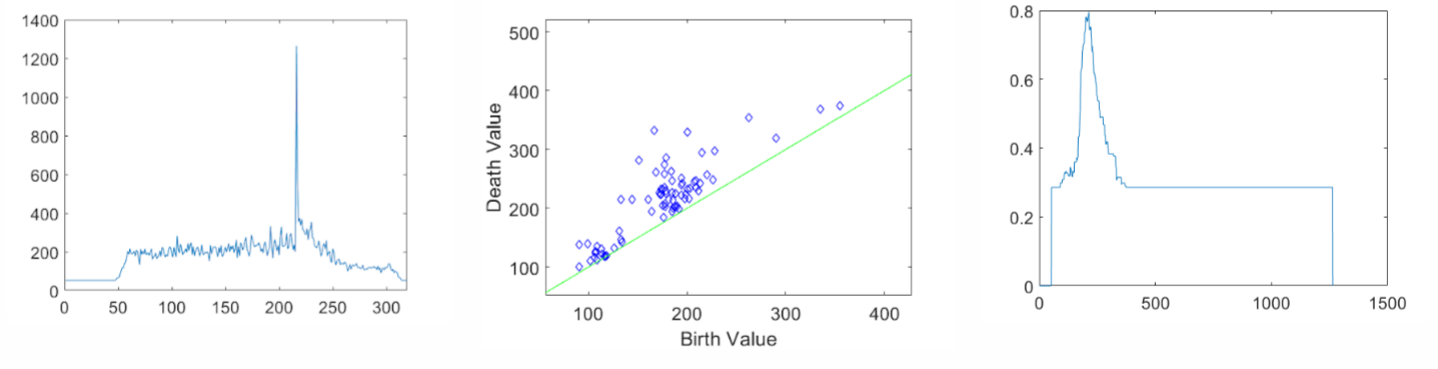
\includegraphics[width=1\textwidth]{figure/持久性曲线2.png} % 请替换为您的第二个图片路径和文件名

    \caption{持久性曲线形成过程}
\end{figure}




\paragraph{持久性中心 (Persistence Centers)}
\label{sec:feat_pcen}
% 原理、文献、优缺点...
与PL和PI试图捕捉PD整体分布不同,严银凯提出的持久性中心(PC)提供了一种更为简洁的表示,它将PD总结为一个(或少数几个)代表性的点。一种具体的定义方式是计算PD中所有点 $(b_i, d_i)$ 的加权平均值,其中权重由持久性 $p_i = d_i - b_i$ 决定。具体地,持久性中心 $\Psi(P_D)$ 可以定义为向量
\begin{equation}
    \Psi(P_D) = \frac{\sum_{x=(b,d) \in P_D} (d-b) x}{\sum_{x=(b,d) \in P_D} (d-b)}
\end{equation}

其中 $x = (b, d) \in \mathbb{R}^2$。
这个计算结果是一个二维向量,可以直观地理解为PD的“重心”,但这里的“质量”被赋予了每个点的持久性。这种表示方法的一个显著优点是其计算极其简单,并且通过持久性加权,它自然地强调了寿命长、结构上更显著的拓扑特征,同时降低了寿命短、可能源于噪声的特征的影响。然而,其代价是极高的信息压缩率,PC几乎丢失了PD中除加权平均位置之外的所有几何分布和结构细节。尽管如此,在某些应用场景下,例如作为后续分类器(如随机森林)的输入特征时,这种高度浓缩的表示可能仍然有效(参考文献\cite{JSJC202406009})。

\paragraph{周期性评分}
Perea等人\cite{perea2015sliding}研究中用于量化时间序列周期性的关键特征是基于其滑动窗口嵌入点云 $X_S$ 的一维持久同调信息。首先,计算 $X_S$ 的Rips复形过滤所导出的一维持久性图 $dgm_1(X_S)$。此图中的每个点 $p=(b,d)$ 代表一个一维拓扑特征(环),其出生尺度为 $b$,死亡尺度为 $d$。该特征的持久性定义为 $pers(p) = d-b$。然后,选取所有这些一维特征中最大的持久性值,即最大持久性 $mp(dgm_1(X_S)) = \max_{(b,d) \in dgm_1(X_S)} \{d-b\}$。最终,将此最大持久性值经过特定缩放,得到周期性评分特征 $Score(X_S)$,在论文的实例中,该评分具体构造为:
\begin{equation}
    Score(X_S) = \frac{mp(dgm_1(X_S))}{\sqrt{3}}
\end{equation}
该标量评分 $Score(X_S)$ 即作为表征原始信号周期强度的特征。
\subsubsection{基于子窗口聚合的鲁棒PH特征提取}
在将持续同调应用于较长时间序列的滑动窗口分析时,研究者常常面临两个主要的实际挑战:其一是,直接处理长窗口数据可能导致持久同调的计算复杂度过高,使得分析效率低下;其二是,长窗口内的时间序列数据更容易受到局部噪声或非典型波动的显著影响,这些干扰可能污染所提取的全局拓扑特征,降低其稳定性和判别能力。针对这些在实际应用中常见的问题,Karan和Kaygun \cite{3} 提出了一种创新性的基于子窗口化(Subwindowing)的拓扑特征提取策略。该策略旨在通过一种分而治之并结合统计聚合的方式,提高拓扑特征对噪声的鲁棒性,并为处理长窗口数据提供一种计算上更高效的途径。

子窗口化方法的核心思想是,对于一个给定的、长度可能较长的主滑动窗口(Main Window)$W_N$,算法并不直接对整个 $W_N$ 进行全局的拓扑分析。取而代之的是,首先将主窗口 $W_N$ 分割为 $M$ 个长度更短、但可能相互重叠的子窗口(Subwindows),记为 $sw_1, sw_2, \dots, sw_M$ [36, 106]。随后,独立的拓扑特征提取过程将在每一个子窗口 $sw_i$ 上分别执行。值得注意的是,Karan和Kaygun在其研究中,为了从每个子窗口中获取更全面的拓扑信息,采用了多角度的分析手段:他们不仅对每个子窗口应用了基于不同嵌入维度(例如,与信号采样频率 $f_s$ 相关的多个特定比例,如 $0.5f_s, 1.0f_s, 1.5f_s, 2.0f_s$ )的时间延迟嵌入并计算相应的持久性图,还额外计算了基于子窗口原始数值序列的上下水平集(upper and lower level set)过滤所产生的持久性图 。通过这种方式,每一个子窗口都对应着一组(在他们的方法中是6个)不同的持久性图,从多个方面刻画了该子片段的拓扑结构。

从每个子窗口的每一个持久性图中,可以进一步提取出一系列基础的拓扑特征描述符。Karan提及他们从每个持久性图的单个同调维度中提取了7种不同的特征,这些特征可能包括基于持久性图上点分布的统计量、基于Wasserstein或Bottleneck距离的度量、持久性熵,或是将持久性图转换为其他表示(如Betti曲线、持久性景观)后再计算其$L^1$或$L^2$范数等 。假设 $f_{i,k}$ 表示从第 $i$ 个子窗口的某个持久性图(或某个特定角度的分析)中提取的第 $k$ 种基础拓扑特征,那么主窗口 $W_N$ 的最终特征向量并不是直接由某个单一分析产生,而是通过统计聚合其内部所有 $M$ 个子窗口的这些基础特征而形成的。该研究中采用的聚合方式主要是计算每种基础特征 $f_{\cdot,k}$ 在所有子窗口上的均值(Mean)和标准差(Standard Deviation)。具体而言,主窗口 $W_N$ 关于第 $k$ 种特征的均值 $\mu_{N,k}$ 计算如下:
\begin{equation}
    \mu_{N,k} = \frac{1}{M} \sum_{i=1}^{M} f_{i,k}
    \label{eq:subwindow_mean}
\end{equation}
而其标准差 $\sigma_{N,k}$ 则由下式给出:
\begin{equation}
    \sigma_{N,k} = \sqrt{\frac{1}{M}\sum_{i=1}^{M}(f_{i,k} - \mu_{N,k})^2} = \sqrt{\left(\frac{1}{M}\sum_{i=1}^{M}f_{i,k}^2\right) - \mu_{N,k}^2}
    \label{eq:subwindow_std}
\end{equation}
通过这种聚合,主窗口的特征不仅概括了其内部拓扑特征的平均表现水平(由均值 $\mu_{N,k}$ 反映),还通过标准差 $\sigma_{N,k}$ 量化了这些拓扑特征在主窗口内部的变异程度或不稳定性 ,这本身也可能成为一项具有判别力的信息。

Karan指出,他们提出的子窗口化策略具有若干显著的优点。首先,该方法能够有效增强拓扑特征对噪声的鲁棒性。现实中的时间序列数据常受到局部噪声或短暂异常波动的干扰,这些干扰若存在于某个子窗口内,其影响会被限制在该子窗口的特征提取结果中。当通过对所有 $M$ 个子窗口的特征进行平均(如公式 \ref{eq:subwindow_mean} 所示)等统计聚合操作时,这些局部的、随机的噪声影响有望被显著平滑或平均掉,从而使得主窗口的最终特征表示更为稳定,更能反映其整体的、持续的拓扑结构。

其次,该策略为处理长主窗口时面临的计算效率问题提供了一种优化途径。持久同调的计算复杂度通常随数据点数的增加而快速增长。若直接对一个非常长的主窗口进行计算,可能会非常耗时。子窗口化将计算分解到多个更短的片段上。更为关键的是,Karan提出了一种高效的滚动更新机制来计算主窗口的聚合特征。当主窗口沿时间序列滑动一个步长时(假设其移出一个最旧的子窗口 $sw_1$,并移入一个新的子窗口 $sw_{M+1}$),新的主窗口 $W_{N+1}$ 的聚合特征(均值和标准差)可以直接根据旧的主窗口 $W_N$ 的聚合特征以及这两个发生变化的子窗口的特征进行递推更新,而无需对所有 $M$ 个子窗口的特征重新进行完整的求和计算。具体地,新的均值 $\mu_{N+1,k}$ 可以表示为:
\begin{equation}
    \mu_{N+1,k} = \mu_{N,k} + \frac{f_{M+1,k} - f_{1,k}}{M}
    \label{eq:recursive_mean}
\end{equation}
同样地,新的方差 $\sigma_{N+1,k}^2$ (标准差的平方) 也可以从旧值递推得到:
\begin{equation}
    \sigma_{N+1,k}^2 = \sigma_{N,k}^2 + (\mu_{N,k}^2 - \mu_{N+1,k}^2) + \frac{f_{M+1,k}^2 - f_{1,k}^2}{M}
    \label{eq:recursive_variance}
\end{equation}
这种递推关系使得在滑动窗口机制下,更新主窗口特征的计算成本在很大程度上与主窗口的实际长度 $M$ 解耦(在子窗口特征已知的前提下,更新的复杂度仅与少数几个变量相关),从而允许研究者在实践中使用较长的主窗口来捕捉更大范围的时间依赖性,而不会导致计算时间的急剧膨胀 。

此外,通过分析子窗口特征的统计分布(如标准差 $\sigma_{N,k}$),该方法还能间接捕捉到一个较长主窗口内部局部动态的变化情况。一个较大的标准差可能意味着主窗口内时间序列的拓扑特性正在经历显著变化,而较小的标准差则可能指示该段序列的拓扑结构相对稳定或均一。

综上所述,Karan提出的基于子窗口聚合的拓扑特征提取策略,通过在更细粒度的子窗口上进行多角度拓扑分析,并结合统计聚合与高效的滚动更新机制,为时间序列的拓扑特征工程提供了一种实用且具有创新性的解决方案。它不仅致力于生成对噪声干扰更为鲁棒的特征表示,还通过巧妙的计算优化,有效应对了处理长段序列时可能面临的计算瓶颈,为基于TDA的时间序列分类及其他相关分析任务提供了有价值的方法论补充。

\subsubsection{PH特征方法比较和讨论}
前文详细介绍了多种从持续同调中构造特征的方法,包括持久性图的统计描述符、基于贝蒂数的表示、多种基于函数或映射的向量化技术(如持久性熵、持久性图像、持久性景观、持久性中心等)以及基于子窗口聚合的鲁棒PH特征提取策略。为更直观地比较这些不同方法在实际应用中的性能表现,表4.1对它们在各自原始研究文献中的关键实验设置、所采用的数据集特性以及主要评估指标和核心结果进行了总结与对比。该表旨在为理解各种PH特征提取方法的有效性和适用场景提供一个实证性的参考。


\begin{center}
    \begin{small} % 使用 small 字号
        % Previous (4 columns): |p{0.18\textwidth}|p{0.24\textwidth}|p{0.26\textwidth}|p{0.28\textwidth}|
        % New (3 columns), removing the 2nd column (参考文献) and redistributing its width (0.24\textwidth)
        % PH特征方法(0.2\textwidth) | 数据集特性(0.35\textwidth) | 评估指标结果(0.4\textwidth)
        \begin{longtable}{|p{0.2\textwidth}|p{0.35\textwidth}|p{0.4\textwidth}|}
            \caption{不同PH特征提取方法在原文献中的实验结果总结} \label{tab:PH_experimental_summary_final_concise}                                                                                                                                                                                                                                                                                                                            \\
            \hline
            \textbf{PH特征方法}                        & \textbf{实验数据集特性}                                                                                                                & \textbf{主要评估指标及结果}                                                                                                                                                                                                                 \\
            \hline
            \endfirsthead

            \multicolumn{3}{c}%
            {{\bfseries 表续:不同PH特征提取方法在原文献中的实验结果总结}}                                                                                                                                                                                                                                                                                                                                                                       \\
            \hline
            \textbf{PH特征方法}                        & \textbf{实验数据集特性}                                                                                                                & \textbf{主要评估指标及结果}                                                                                                                                                                                                                 \\
            \hline
            \endhead

            \hline \multicolumn{3}{|r|}{{续下一页}}                                                                                                                                                                                                                                                                                                                                                                           \\
            \endfoot

            \hline
            \endlastfoot

            持久性图的统计描述符\cite{mittal2017topological} & 1. Logistic映射 (含噪声时间序列)。\newline 2. Duffing振子 (含噪声时间序列,经去噪)。\newline 3. Op-amp Jerk电路 (含噪声时间序列,经去噪)。                            & 提取的拓扑特征($nrel_k, avg_k, K_{orbit}, D_i$等)随系统参数变化的趋势图显示其在分岔点和混沌起始点有清晰指示能力,优于或补充了LLE、排列熵、关联维等传统指标。计算时间 < 4分钟。                                                                                                                        \\
            \hline
            基于Betti数的表示\cite{umeda2019topological} & 1. 分类: 人体活动传感器数据(陀螺仪、EEG、EMG)。\newline 2. 异常检测: 桥梁振动数据。                                                                         & Betti序列 + 1D CNN。\newline 分类准确率: 对比SVM+传统特征,准确率提升 >20\%。\newline 异常检测(桥梁): 拓扑指标“异常度”与实际损伤吻合,可早期预警。                                                                                                                                 \\
            \hline
            持久性熵 (PE)\cite{atienza2020stability}   & 1. PE区分能力: 正态 vs 均匀分布点云。\newline 2. 鲁棒性: USC-SIPI图像(加多种噪声)。\newline 3. 分类: FMD材质图像(10类及成对)。                                     & PE区分能力: Mann-Whitney U检验 $p=0.046$。\newline 鲁棒性($L_1$距离): NES函数(基于PE)对高斯/泊松噪声优于Betti曲线。\newline FMD分类(随机森林准确率): 10分类Betti+NES组合最高(0.29);成对分类中PI和Betti常更优。                                                                          \\
            \hline
            持久性图像 (PI)\cite{adams2017persistence}  & 1. 合成形状分类: 6类拓扑空间点云(含噪声)。\newline 2. 耦合扭转映射: 离散动力系统点云。\newline 3. aKS方程: PDE表面数据。                                               & K-medoids分类准确率(合成形状): PI (如$H_1, L^\infty, \eta=0.1$: 96.0\%),计算时间优于PDs。\newline PI参数选择不敏感。SSVM特征选择后准确率100\%。\newline 耦合扭转映射分类($H_0+H_1$ PIs): 准确率82.5\%。\newline aKS方程参数分类($H_0+H_1$ PIs, $t=10$): 准确率97.3\%。                     \\
            \hline
            持久性景观 (PL)\cite{1}                     & 1. 关联环体: 100次采样。\newline 2. 高斯随机场(GRF): $[0,1]^2$和$[0,1]^3$上,100样本。\newline 3. 圆环 vs. 球面: 实验A(无噪声, 100样本/类);实验B(加高斯噪声, 10样本/类)。 & 统计检验p值。\newline 圆环 vs. 球面(无噪声): $H_1$景观积分z检验显著区分($p=3\times10^{-6}$)。\newline 圆环 vs. 球面(有噪声): 均值景观间$L^2$距离置换检验,$H_0, H_1, H_2$均显著区分 ($p \le 0.0111$)。                                                                              \\
            \hline
            基于子窗口聚合的鲁棒PH特征\cite{3}                 & 1. 合成数据集: 模拟生理信号(RESP, ECG)区分压力与非压力。\newline 2. WESAD数据集: 真实多模态生理信号,3分类。\newline 3. DriveDB数据集: 真实生理信号,3分类。                     & 分类准确率, $F_1$-score (LOSOCV)。\newline 合成数据(SVM): 近乎完美区分。\newline WESAD (60s窗口, SVM): 三分类最高81.35\% ($F_1$=73.44\%);二分类最高94.46\% ($F_1$=93.26\%)。\newline DriveDB (60s窗口): 三分类最高85.81\% ($F_1$=79.68\%);二分类最高98.07\% ($F_1$=97.97\%)。 \\
            \hline
        \end{longtable}
    \end{small}
\end{center}


\subsection{时间序列的其他特征}
\label{sec:other_ts_features}
% 核心:介绍非TDA的时间序列特征提取和度量方法。
在上文我们介绍了采用持续同调方法提取时间序列的拓扑特征,本小节旨在系统性的梳理和介绍拓扑数据分析之外的其他特征提取方法.拓扑特征能够捕捉时间序列数据的全局形状和连接性信息,但它们可能无法完全捕捉到数据的其他重要方面,例如局部统计特性,频率成分或特定的子序列模式。因此,探索和理解补充性的非拓扑特征对于构建更全面、更强大的TSC模型至关重要。这种对拓扑特征之外方法的探索需求本身就体现了一个重要的认知:没有任何单一类型的特征能够捕获时间序列中所有相关的信息。文献中将特征划分为统计特征、频域特征、时域特征(包括基于距离和形状的方法)、基于模型的特征以及深度学习自动提取的特征等多个类别 ,这进一步印证了采用多样化特征集来捕捉时间序列不同方面动态的必要性。
\subsubsection{时域统计特征}
\label{sec:ts_distances}
% DTW, 编辑距离等...
统计特征提取是最基础也是最常用的时间序列特征化方法之一。这类特征主要基于时间序列值的整体分布特性和基本的时间依赖关系进行描述。

基本的描述性统计量\cite{box2015time}概括了时间序列值的集中趋势、离散程度和分布形状。衡量数据中心位置的指标包括均值(Mean)、中位数(Median)和截尾均值(Trimmed Mean)。算术平均值可以代表物理系统的操作点或工作点,但对异常值非常敏感。在存在显著异常值的情况下,中位数和截尾均值是更稳健的选择。自动化库如 tsfresh\cite{christ2018time} 通常包含均值特征。衡量数据点围绕均值的离散程度或波动性的指标是方差(Variance)和标准差(Standard Deviation)。方差越大,表示数据波动越剧烈。tsfresh 也包含这些特征。

分布形状的度量包括偏度(Skewness)和峰度(Kurtosis)。偏度衡量时间序列振幅概率密度函数(PDF)的对称性。偏度为零表示对称分布;正偏度(右偏)表示存在许多小值和少量大值;负偏度(左偏)表示存在许多大值和少量小值。偏度的变化可能指示相关物理系统的系统性变化。tsfresh 库计算偏度。峰度则衡量时间序列振幅PDF的“尖峰”程度。接近3的峰度值表示类似高斯分布的尖峰度。大于3表示相对尖锐的峰(尖峰),小于3表示相对平坦的峰(平峰)。峰度的变化同样可以反映系统的变化。tsfresh 库计算峰度。

此外,最小值(Minimum)和最大值(Maximum)表示时间序列中的极端值,tsfresh 包含这些极值特征。分位数(Quantiles)指示数据分布中特定百分比位置的值,例如四分位数、百分位数等,tsfresh 也可以提取分位数特征。这些基本的统计特征可以通过 pandas、numpy 和 scipy.stats 等 Python 库方便地计算,而 tsfresh 等自动化库则能够自动计算其中的许多特征。

自相关特征\cite{barnard2001embedding}描述了时间序列与其自身在不同时间滞后(lag)版本之间的关系。自相关函数(Autocorrelation Function, ACF)测量时间序列与其滞后版本之间的相似度。ACF图常用于识别数据中的重复模式或季节性。例如,如果ACF在滞后12处出现显著峰值,可能表示存在年度季节性。tsfresh 可以计算聚合的自相关特征,例如不同滞后下的自相关系数的均值或方差。偏自相关函数(Partial Autocorrelation Function, PACF)测量序列与其滞后版本之间的相关性,同时控制(移除)了中间滞后的影响。PACF对于识别自回归(AR)模型的阶数特别有用。tsfresh 也提供了偏自相关系数的计算。


自动化库 tsfresh 提供了大量预定义的统计特征,除了上述提及的,还包括例如:绝对能量(Absolute Energy),即时间序列值的平方和 $\sum_{i=1}^{n} x_i^2$;绝对变化均值(Mean Absolute Change),即连续值之间绝对差值的平均值 $\frac{1}{n-1}\sum_{i=1}^{n-1} \lvert x_{i+1} - x_i \rvert$;峰值数量(Number of Peaks),计算时间序列中局部最大值的数量,可以指定峰值所需的最小支持邻域。此外,tsfresh 还包含多种熵度量(Entropy Measures),如基于值分箱计算熵的分箱熵(Binned Entropy),基于功率谱密度的傅里叶熵(Fourier Entropy),基于相邻值排序模式复杂性的排列熵(Permutation Entropy),衡量规律性的样本熵(Sample Entropy),以及衡量可预测性和复杂性的近似熵(Approximate Entropy)。

虽然这些基本的统计特征是理解时间序列的基础,并且计算相对简单,但它们主要捕捉的是线性依赖关系(如ACF)和整体的分布属性。它们可能难以捕捉到数据中复杂的非线性动态、瞬态事件或基于形状的模式。例如,一个具有复杂周期性或混沌行为的序列,其均值和方差可能无法完全反映其动态特性。这就引出了对更高级特征提取方法的需求,例如频域分析、形状分析和深度学习方法,这些方法将在后续章节中讨论。

\subsubsection{频域特征}
\label{sec:ts_statistical_spectral}
% 时域统计量,频域特征...
频域分析\cite{yi2023survey}是将时间序列从时域转换到频域,以揭示其周期性成分和频谱特性的重要方法。这种转换有助于识别在时域中不明显的重复模式或振荡行为。

基于傅里叶变换(Fourier Transform, FT)的特征是一种经典方法。傅里叶变换是一种信号处理技术,它将一个信号分解为其组成的正弦和余弦波的总和,每个波对应一个特定的频率。其核心思想是任何(足够规则的)周期信号都可以表示为不同频率和振幅的正弦波的叠加。对于时间序列分析,通常使用离散傅里叶变换(Discrete Fourier Transform, DFT)或其快速算法——快速傅里叶变换(Fast Fourier Transform, FFT)。傅里叶变换在频域提供了高分辨率,但在时域没有分辨率,这意味着它可以精确地告诉我们信号中存在哪些频率,但不能告诉我们这些频率在时间上的具体位置。因此,它最适用于分析频率成分不随时间变化的平稳信号。

从傅里叶变换中可以提取多种特征。DFT/FFT 的输出是一系列复数形式的傅里叶系数(Fourier Coefficients),每个系数对应一个特定的频率。这些系数的振幅(Magnitude)表示该频率分量的强度,相位(Phase)表示该频率分量的起始位置。可以直接使用某些频率的系数(或其振幅/相位)作为特征。tsfresh 库可以提取特定系数的实部、虚部、绝对值或角度作为特征。功率谱密度(Power Spectral Density, PSD)描述了信号功率如何随频率分布,它通常通过周期图(Periodogram)来估计,即傅里叶变换系数模平方的一种度量。PSD可以揭示信号中的主导频率,tsfresh 提供了基于Welch方法估计的PSD特征。频谱熵(Spectral Entropy)是基于PSD计算的熵值,衡量频谱的平坦度或复杂度。低频谱熵表示信号能量集中在少数频率上(可预测性高),高频谱熵表示能量分布广泛(更接近白噪声,可预测性低);tsfresh 计算傅里叶熵(一种基于分箱的频谱熵)。频谱矩(Spectral Moments),如频谱质心(平均频率)、频谱方差(频率分布宽度)、频谱偏度、频谱峰度等,描述了频谱的整体形状,tsfresh 通过 fft\_aggregated 函数提取这些特征。频谱中的主导频率或峰值(Dominant Frequencies/Peaks)通常对应于信号中最显著的周期性成分。近年来,有研究开始探索直接在傅里叶域中对时间序列进行建模,例如神经傅里叶建模(Neural Fourier Modelling, NFM),认为这是一种紧凑且强大的时间序列分析方法,适用于预测、异常检测和分类等任务。这种方法利用傅里叶变换将有限长度时间序列视为函数空间中的连续时间元素,并允许在频域内进行重采样等操作。

为了克服傅里叶变换在分析非平稳信号(即频率成分随时间变化的信号)时的局限性,发展了基于小波变换(Wavelet Transform, WT)的特征提取方法。与傅里叶变换使用无限长的正弦波作为基函数不同,小波变换使用具有有限持续时间和特定形状的“母小波”(Mother Wavelet)及其伸缩(Dilation)和平移(Translation)版本作为基函数。这使得小波变换能够同时提供时间和频率(或尺度)的信息,实现时频局部化分析,特别适合分析包含瞬态事件、频率随时间变化的非平稳信号。

小波变换\cite{rhif2019wavelet}主要有两种形式。连续小波变换(Continuous Wavelet Transform, CWT)通过连续地伸缩和平移母小波来分析信号,提供非常详细的时频表示。其结果通常可视化为时频图,称为尺度图(Scalogram),显示了不同时间和尺度(对应频率)上的小波系数强度;tsfresh 可以提取CWT系数。离散小波变换(Discrete Wavelet Transform, DWT)则通过一系列高通和低通滤波器(滤波器组)对信号进行分解,通常采用二进尺度和位置。在每个分解层级(level),DWT将信号分解为近似系数(Approximation Coefficients,低频成分,代表信号的平滑部分或趋势)和细节系数(Detail Coefficients,高频成分,代表信号的细节或快速变化)。这个过程可以递归地应用于近似系数,从而得到多层分解,每一层对应不同的频率范围;sktime 库\cite{loning2019sktime}提供了 DWTTransformer,默认使用Haar小波进行分解。

从小波变换中提取特征的方式也多种多样。DWT产生的近似系数和各层细节系数本身可以作为特征,因为它们捕获了信号在不同时间和频率尺度上的信息。然而,由于小波系数的数量可能仍然很大,通常的做法是从每个分解层级(或称为子带, sub-band)的系数中提取统计特征,如均值、方差、标准差、能量、熵等。例如,可以计算每个细节系数子带的方差,以量化信号在不同频率段的波动性。tsfresh 库也提供了计算小波系数统计量的功能。

在使用小波变换时,需要选择合适的母小波和分解层数。母小波的选择取决于其形状特性(如对称性、紧支撑性)与待分析信号特征的匹配程度。分解层数的选择则关系到所能分析的最低频率和时频分辨率的权衡。这些选择往往需要领域知识或通过实验进行调整。例如,sktime 的 DWTTransformer 默认使用最简单的Haar小波,但其他库(如PyWavelets)或更高级的应用可能需要选择更复杂的母小波。

频域分析提供了一种与时域分析互补的视角。傅里叶变换是分析平稳周期性信号的有力工具,而小波变换则为分析具有时变频率特性或瞬态事件的非平稳信号提供了强大的时频局部化能力。两者之间的关键区别在于对信号平稳性的要求以及时频分辨率的权衡。傅里叶变换提供精确的频率信息但牺牲了时间信息,适用于频率成分固定的信号;小波变换则在时间和频率分辨率之间取得平衡,更适合分析动态变化的信号。无论是傅里叶系数还是小波系数,其数量都可能非常庞大。因此,在实际应用中,通常不是直接使用所有原始系数作为特征,而是对这些系数进行进一步处理,如计算系数的统计摘要(频谱熵、小波系数能量、子带方差等),或者将整个变换结果(如尺度图)视为一个整体输入到另一个机器学习模型(特别是CNN)中进行更高层次的特征学习。这种处理方式引入了抽象层级,使得最终特征代表了更复杂的频谱或时频模式。虽然小波变换功能强大,但其应用也引入了选择母小波和分解层数的复杂性,这与傅里叶变换相对标准化的应用形成了对比。

\subsubsection{时域模式和形状特征}
\label{sec:ts_subsequence_pattern}
% Shapelets, Bag-of-Words/Symbolic...
时域特征提取直接从时间序列的原始数值序列中进行,重点关注数据点之间的时间顺序、局部模式、形状以及滞后关系。

利用时间序列的先前值来构建当前或未来值的预测特征是连接时间序列分析和监督学习的关键桥梁,这通常通过滞后与窗口特征实现。滞后特征(Lag Features)是最基本的思想,即使用过去某个时间点(如 $t-1, t-2, \dots$)的值 $x_{t-1}, x_{t-2}, \dots$ 作为预测当前或未来时间点(如 $t$ 或 $t+1$)值 $x_t$ 或 $x_{t+1}$ 的特征。这可以通过 pandas 库中的 \texttt{shift()} 函数轻松实现,该函数将序列向下移动指定的步数。通过包含多个滞后值作为输入特征,可以构建更复杂的模型。选择包含多少个滞后值(即窗口宽度)通常需要实验确定,并可能依赖于数据的自相关性。对于具有季节性的数据,还可以考虑包含更长周期的滞后值。

滑动窗口特征(Rolling/Sliding Window Features)\cite{3}计算先前固定大小时间窗口内的值的摘要统计量,而不是直接使用滞后值。例如,可以使用过去5个时间点的平均值作为当前点的特征。常见的统计量包括均值、中位数、标准差、最小值、最大值等。这种方法有助于平滑噪声并捕捉局部趋势。pandas 的 \texttt{rolling()} 函数可以创建滑动窗口对象,然后在其上应用各种聚合函数(如 \texttt{.mean()}, \texttt{.std()})来生成特征。扩展窗口特征(Expanding Window Features)与滑动窗口不同,它包含从序列开始到当前时间点的所有先前数据。基于扩展窗口计算的统计量(如累积均值、累积最大值)可以捕捉全局或累积性的信息,pandas 的 \texttt{expanding()} 函数用于此目的。在使用时,通常需要将序列 \texttt{shift(1)} 以确保用于生成特征的窗口不包含当前要预测的值。滞后和窗口特征是构建监督学习模型的基础,但它们主要捕捉的是基于固定时间间隔的依赖关系或局部统计汇总,对于需要识别特定形状模式或处理时间轴扭曲的情况,则需要更专门的方法。

基于Shapelet的特征是另一种重要的时域方法。Shapelet方法的核心思想是在时间序列中寻找能够最好地区分不同类别的代表性子序列(即Shapelet)。分类决策基于一个时间序列与这些已发现的Shapelet的相似程度(通常用距离度量)。Shapelet是时间序列中的一个连续子序列,它对预测目标变量(类别标签)具有最大的区分能力。例如,在心电图(ECG)分类中,某个特定形状的波形段可能只出现在患有某种心脏病的患者的ECG序列中,这个波形段就可以作为一个Shapelet。Shapelet方法的一个主要优点是其可解释性:找到的Shapelet本身就是原始数据的一部分,可以直观地理解其代表的模式,为领域专家提供洞察。

Shapelet变换(Shapelet Transform)是一种常用的利用Shapelet进行分类的方法。其过程包括:首先,从训练数据中搜索并选择出 $k$ 个最具区分能力的Shapelet,这通常涉及评估大量候选子序列区分不同类别的能力(例如,通过信息增益或F统计量);其次,对于数据集中的每个时间序列,计算它到这 $k$ 个选定Shapelet的最小距离(通常定义为Shapelet与该时间序列中所有等长子序列之间距离的最小值),从而将每个原始时间序列转换成一个 $k$ 维的特征向量;最后,使用这个转换后的特征向量和原始标签来训练任何标准的分类器(如支持向量机SVM、随机森林、旋转森林等)。Shapelet算法存在多种变种,包括将Shapelet发现嵌入决策树构建的方法、通过优化算法同时学习Shapelet形状和分类器权重的学习Shapelet(Learning Shapelets, LS)、为提高效率随机采样候选Shapelet的方法(常与集成方法结合,如Random Shapelet Forest),以及结合卷积思想允许Shapelet跳点匹配以捕捉不同时间尺度模式的扩张Shapelet(Dilated Shapelets, 如DST, Castor)。Shapelet与时间序列之间的距离通常使用z标准化的欧氏距离(z-normalized Euclidean distance)计算,以消除基线漂移和振幅缩放的影响,但也可以使用动态时间规整(DTW)作为距离度量(如LTSD方法)来处理时间轴扭曲。sktime 和 pyts 等库提供了Shapelet变换的实现。

动态时间规整(Dynamic Time Warping, DTW)本身也是一种强大的时域分析工具,主要用于测量两个可能在时间轴上发生扭曲或变速的时间序列之间的相似性。DTW通过寻找两条时间序列之间的最优非线性对齐路径(warping path)来计算它们之间的距离。它允许一个点与另一个序列中的多个点对齐,从而有效地处理时间序列之间的局部拉伸、压缩或相位移动,这是欧氏距离无法做到的。DTW距离是沿着这条最优路径累积的对应点之间的距离(通常是平方距离)的总和(或其平方根),通常使用动态规划算法找到最优路径。

DTW最直接的应用是作为时间序列的距离度量,与k-近邻(k-NN)分类器结合使用,特别是1-NN DTW,曾被认为是时间序列分类(TSC)领域的基准方法。此外,DTW距离本身也可以用于特征提取。一种创新的方法是计算一个待分类时间序列与训练集中每一个时间序列的DTW距离,这些距离构成一个特征向量,输入到标准分类器中(如SVM)。这种方法利用了DTW捕捉相似性的能力,并将其与更强大的分类模型结合。同时,如前所述,DTW也可以替代欧氏距离,在Shapelet算法中计算Shapelet与时间序列的距离。DTW的主要缺点是其较高的计算复杂度,对于长度为 $n$ 和 $m$ 的序列,复杂度为 $O(nm)$(等长序列为 $O(n^2)$),远高于欧氏距离的 $O(n)$。这使得DTW在处理大规模数据集或长序列时效率低下。为缓解此问题,常使用约束(如Sakoe-Chiba带或Itakura平行四边形)限制搜索范围,或使用近似算法(如FastDTW、PrunedDTW),尽管可能牺牲最优性。多个Python库如 dtaidistance 和 tslearn 实现了DTW及其变种,sktime 也在其距离模块和分类器中集成了DTW。

时域特征提取方法提供了多种捕捉时间序列动态的方式。滞后和窗口特征侧重于基于固定时间偏移或窗口的统计汇总和线性依赖关系。相比之下,Shapelet和DTW方法则侧重于模式匹配和形状相似性,能够处理相位独立性和时间扭曲。这种关注点的差异——统计聚合 vs. 模式/形状相似性——使得它们适用于不同类型的时间序列特性。在可解释性方面,Shapelet因其能够提供直观的、源自数据的模式而备受推崇。滞后和窗口特征也相对容易解释。然而,基于DTW距离的特征(即到所有训练样本的距离向量)维度可能很高,其解释性不如Shapelet直接,更像是基于样本在DTW距离空间中的相对位置进行分类。计算成本方面存在明显的层级:滞后/窗口特征通常最快(线性扫描);DTW计算成本高(二次或约束下的超线性);Shapelet发现也可能非常耗时,尽管随机化和变换方法等优化措施旨在降低这一成本。





\subsection{基于特征的时间序列分类}
一旦时间序列被转化为了一个特征向量,原始的序列分类问题就转化为了一个更加标准的模式识别任务。
此时,我们就可以使用多种标准的机器学习分类器,这些分类器在模式识别领域有这广泛的应用和成熟的理论基础。下面介绍一些常见的分类算法。

\paragraph*{K-近邻 (k-NN)}
k-NN算法的核心思想是:一个样本的类别由其在特征空间中最近的k个邻居的多数类别决定 。在应用k-NN时,关键的考虑因素包括邻居数量k的选择以及距离度量的选择。对于特征向量,欧氏距离是常用的度量方式。值得注意的是,k-NN对特征的尺度非常敏感,因此在应用前通常需要进行特征缩放。在持续同调领域,有研究直接将1-NN分类器与持久性曲线或基于持久性图的度量相结合 。\cite{susto2018time}

\paragraph*{支持向量机 (SVM)}
SVM旨在特征空间中找到一个能够以最大间隔将不同类别分开的最优超平面 。通过引入核技巧(如线性核、多项式核、径向基函数(RBF)核),SVM能够有效地处理非线性可分的数据。SVM在处理高维特征时表现良好,但在选择合适的核函数及其参数(如正则化参数C)方面需要仔细调整。
\cite{de2023persistent}

\paragraph*{决策树和集成方法}
决策树通过学习一系列简单的决策规则来构建树状结构,易于理解和解释。然而,单个决策树很容易过拟合训练数据。随机森林作为一种集成学习方法,通过构建并组合多颗决策树的预测结果来提升分类性能并减少过拟合,通常具有较强的鲁棒性。梯度提升机例如XGBoost和LightGBM等,通过迭代地训练弱分类器(通常是决策树)来优化损失函数,具有较高的准确性和效率。集成方法在处理高维特征时表现良好,但需要注意模型的复杂性和训练时间。

\begin{table}[h!]
    \centering
    \caption{用于已提取时间序列特征的常用分类器概述}
    \label{tab:classifiers_condensed}
    \begin{tabular}{|p{2cm}|p{3.5cm}|p{4cm}|p{4.5cm}|}
        \hline
        \textbf{分类器名称}                            & \textbf{简要描述}                         & \textbf{主要优势}                 & \textbf{主要考量/局限性}                        \\
        \hline
        k-近邻 (k-NN)                               & 基于特征空间中k个最近邻居的多数类别进行分类。               & 实现简单,对数据分布无假设,非线性。            & 计算成本高(预测阶段),对特征缩放敏感,需选择合适的k值和距离度量。       \\
        \hline
        支持向量机 (SVM)                               & 在特征空间中寻找一个最优超平面来分离类别;核技巧可实现非线性分离。     & 在高维空间中有效,对过拟合有较好鲁棒性,可选择不同核函数。 & 对参数选择(如C值、核函数参数)敏感,对缺失数据敏感,大规模训练集计算复杂度高。 \\
        \hline
        随机森林 (RF)                                 & 决策树的集成,通过构建多棵决策树并综合其预测结果来进行分类,减少过拟合。  & 鲁棒性强,能处理高维数据,不易过拟合,能评估特征重要性。  & 对于某些噪声较大的数据集可能会过拟合,模型解释性相对较差(相比单决策树)。    \\
        \hline
        梯度提升机 (GBM) (XGBoost, LightGBM, CatBoost) & 顺序构建决策树,每棵树都试图纠正前一棵树的错误,通常在表格数据上表现优异。 & 预测精度高,能处理各种类型的特征,内置正则化防止过拟合。  & 训练时间可能较长,对超参数敏感,模型可解释性较差。                \\
        \hline
    \end{tabular}
\end{table}






\subsection{实验设计}
本文在第二章和第三章详细的列举了时间序列分类算法的相关背景和持续同调的应用背景,再结合第四章的特征提取方法,本文基于上述内容设计了一个实验来验证基于持续同调的时间序列分类方法的有效性。

\subsubsection{数据集}
UCR时间序列数据集\cite{UCRArchive2018}是一个由加州大学河滨分校维护和发布的综合性基准数据集。它的建立旨在为时间序列分类算法的开发与评估提供一个标准化平台。

该数据集的历史可以追溯到2002年,最初版本包含了16个时间序列数据集。随着时间序列数据挖掘研究的不断深入,UCR数据集也在持续发展和完善。至2015年,其规模扩展至85个数据集,并经过了严格的标准化和去噪处理,进一步提升了数据集的质量和可用性。到了2018年,数据集的数量再次大幅增加,达到了128个独立的时间序列数据集。这些数据集涵盖了生物医学、图像、音频、金融、运动识别等多个领域,序列长度和类别数量各异,极大地丰富了研究的广度。UCR数据集的持续更新与维护,使其成为时间序列分析领域最具影响力的开源资源之一,被全球范围内的研究人员广泛引用和使用。

在应用方面,UCR时间序列数据集主要作为时间序列分类算法性能评估的基准。研究人员利用UCR数据集来验证其新算法的有效性、鲁棒性以及泛化能力。由于提供了统一的训练集和测试集划分标准,不同算法可以在相同的数据集上进行公平的比较,这对于推动时间序列分类领域的进步至关重要。无论是传统的基于距离的方法(如DTW-KNN)、基于特征的方法(如Shapelet)还是新兴的基于深度学习的方法(如卷积神经网络、循环神经网络、Transformer等),UCR数据集都是其性能验证和比较的重要实验平台。此外,UCR数据集的领域多样性也促使研究人员探索时间序列分析在不同实际应用场景中的潜力,从而将理论研究成果转化为解决实际问题的有效工具。下面的表格展示本文使用的部分UCR数据集的基本信息。
%这里预留一下表格位置

\begin{table}[h!]
    \centering
    \caption{多变量时间序列分类数据集档案选例}
    \label{tab:multivariate_tsc_archive}
    \begin{tabular}{lccccc} % 删除了"旧长度"列,并调整了列数
        \toprule
        \textbf{数据集}          & \textbf{长度} & \textbf{类别数} & \textbf{维度} & \textbf{训练样本} & \textbf{测试样本} \\
        \midrule
        ArabicDigits          & 93          & 10           & 13          & 6600          & 2200          \\
        AUSLAN                & 136         & 95           & 22          & 1140          & 1425          \\
        CharacterTrajectories & 205         & 20           & 3           & 300           & 2558          \\
        CMUsubject16          & 580         & 2            & 62          & 29            & 29            \\
        ECG                   & 152         & 2            & 2           & 100           & 100           \\
        JapaneseVowels        & 29          & 9            & 12          & 270           & 370           \\
        KickVsPunch           & 841         & 2            & 62          & 16            & 10            \\
        Libras                & 45          & 15           & 2           & 180           & 180           \\
        Outflow               & 997         & 2            & 4           & 803           & 534           \\
        UWave                 & 315         & 8            & 3           & 200           & 4278          \\
        Wafer                 & 198         & 2            & 6           & 298           & 896           \\
        WalkVsRun             & 1919        & 2            & 62          & 28            & 16            \\
        \bottomrule
    \end{tabular}
\end{table}

这些数据集的长度在29-1919之间,而且涵盖了多个类别数,遵循数据集给定的划分将其分为训练集和测试集,并在这些数据集上面进行算法的评估的比较。这样的数据集选择和处理使得实验具有一定的可靠性,能够较好的评估算法的性能。
\subsubsection{实验设置}
本节实验依托的是Fawaz等人\cite{ismail2019deep}开源的github仓库项目,该作者详细地介绍了如何利用深度学习进行时间序列分类,本文在它的基础上加入了自己利用持续同调获取到的特征进行分类的实验。

实验数据预处理始于对原始数据集 $D=\left\{\boldsymbol{y}_1, \boldsymbol{y}_2, \cdots, \boldsymbol{y}_m\right\}$ 执行 Min-Max 归一化。此步骤生成了转换后的数据集 $D^{\prime}=\left\{\hat{\boldsymbol{y}}_1, \hat{\boldsymbol{y}}_2, \cdots, \hat{\boldsymbol{y}}_m\right\}$,其中每个 $\hat{\boldsymbol{y}}_i=\left(\hat{y}_{i, 0}, \hat{y}_{i, 1}, \cdots, \hat{y}_{i, n}\right)$ 均为长度为 $n+1$ 的单变量时间序列。然而,将这些原始时间序列直接视为 $n$ 维向量难以揭示其固有的高维拓扑结构。因此,对时间序列数据进行重构以提取更深层次的信息显得尤为重要。

接着,我们引入一个映射 $f: \mathbb{R}^{n+1} \rightarrow \mathbb{R}^{2 \times n}$,其定义如下:

$$
    \begin{aligned}
         & f\left(\hat{\boldsymbol{y}}_i\right)=f\left(\hat{y}_{i, 0}, \hat{y}_{i, 1}, \cdots, \hat{y}_{i, n}\right)=        \\
         & \left(\boldsymbol{q}_{i, 1}, \boldsymbol{q}_{i, 2}, \cdots, \boldsymbol{q}_{i, n}\right), i \in\{1,2, \cdots, m\}
    \end{aligned}
$$

这里,$\boldsymbol{q}_{i, j}=\left(\hat{y}_{i, 0}, \hat{y}_{i, j+1}-\hat{y}_{i, j}\right) \in \mathbb{R}^2$,适用于 $j \in\{1,2, \cdots, n-1\}$。通过这种转换,原始时间序列 $\hat{\boldsymbol{y}}_i$ 被投影到新的 $\mathbb{R}^{2 \times n}$ 空间中。由此产生的序列 $\left(\boldsymbol{q}_{i, 1}, \boldsymbol{q}_{i, 2}, \cdots, \boldsymbol{q}_{i, n}\right)$ 可被视为一个由 $n$ 个点组成的点云,其中每个 $\boldsymbol{q}_{i, j}$ 对应于该点云上的一个具体点 $\left(\hat{y}_{i, 0}, \hat{y}_{i, j+1}-\hat{y}_{i, j}\right)$。这种转换使得每个时间序列都能够对应一个独特的点云,从而为后续的拓扑数据分析奠定了基础。
在点云的基础上,我们进一步计算其持久性同调(PH)特征。具体而言,我们使用 ripser 库来计算持久性图(PD),并利用 GUDHI 库来提取持久性同调特征。我们选择了持续同调的维度 $k=0,1,2$,并将其持久性图转换为持久性图像(PI)和持久性景观(PL)。这些拓扑特征被用作后续分类器的输入。

我们利用配置好的相关深度学习网络,修改输入参数,在docker平台上运行了深度学习模型。本实验的相关设备是:CPU是英特尔酷睿i7-12700H,内存是32GB,GPU是NVIDIA GeForce RTX 3060,显存是6GB。在不同的网络分类器结果如下所示:

\begin{table}[h!]
    \centering
    \caption{各模型在多变量时间序列分类数据集上的准确率}
    \label{tab:model_performance_multivariate_tsc}
    \begin{tabular}{lcccccc}
        \toprule
        \textbf{数据集}          & \textbf{PHMLP} & \textbf{PHFCN} & \textbf{MLP} & \textbf{FCN} & \textbf{MCNN} & \textbf{t-LeNet} \\ % 删除了MCDCNN列
        \midrule
        AUSLAN                & 93.3(0.5)      & 97.5(0.4)      & 97.4(0.3)    & 93.8(0.5)    & 1.1(0.0)      & 1.1(0.0)         \\
        ArabicDigits          & 96.9(0.2)      & 99.4(0.1)      & 99.6(0.1)    & 98.1(0.1)    & 10.0(0.0)     & 10.0(0.0)        \\
        CMUsubject16          & 60.0(16.9)     & 100.0(0.0)     & 99.7(1.1)    & 98.3(2.4)    & 53.1(4.4)     & 51.0(5.3)        \\
        CharacterTrajectories & 96.9(0.2)      & 99.0(0.1)      & 99.0(0.2)    & 97.1(0.2)    & 5.4(0.8)      & 6.7(0.0)         \\
        ECG                   & 74.8(16.2)     & 87.2(1.2)      & 86.7(1.3)    & 87.2(0.8)    & 67.0(0.0)     & 67.0(0.0)        \\
        JapaneseVowels        & 97.6(0.2)      & 99.3(0.2)      & 99.2(0.3)    & 97.6(0.6)    & 9.2(2.5)      & 23.8(0.0)        \\
        KickvsPunch           & 61.0(12.9)     & 54.0(13.5)     & 51.0(8.8)    & 61.0(9.9)    & 54.0(9.7)     & 50.0(10.5)       \\
        Libras                & 78.0(1.0)      & 96.4(0.7)      & 95.4(1.1)    & 78.3(0.9)    & 6.7(0.0)      & 6.7(0.0)         \\
        NetFlow               & 55.0(26.1)     & 89.1(0.4)      & 62.7(23.4)   & 77.7(0.5)    & 77.9(0.0)     & 72.3(17.6)       \\
        UWave                 & 90.1(0.3)      & 93.4(0.3)      & 92.6(0.4)    & 90.8(0.4)    & 12.5(0.0)     & 12.5(0.0)        \\
        Wafer                 & 89.4(0.0)      & 98.2(0.5)      & 98.9(0.4)    & 98.6(0.2)    & 89.4(0.0)     & 89.4(0.0)        \\
        WalkvsRun             & 70.0(15.8)     & 100.0(0.0)     & 100.0(0.0)   & 100.0(0.0)   & 75.0(0.0)     & 60.0(24.2)       \\
        \midrule
        Average Rank          & 5.21           & 2.00           & 2.88         & 3.04         & 7.58          & 8.00             \\
        \bottomrule
    \end{tabular}
\end{table}
由上表可知,在结合了PH特征后,PHMLP和PHFCN模型在大多数数据集上都取得了显著的性能提升。尤其是在AUSLAN、ArabicDigits和CharacterTrajectories等数据集上,PHMLP和PHFCN的准确率均超过了95\%。在CMUsubject16数据集上,PHMLP的表现略逊于其他模型,但仍然达到了60\%的准确率。整体来看,PH特征在多变量时间序列分类任务中展现出了良好的性能,证明了持续同调方法在时间序列分析中的有效性。下面是算法的伪代码,展示了如何利用持续同调特征进行时间序列分类。

\begin{comment}
    

\begin{algorithm}[H]
    \caption{基于持续同调的时间序列分类}
    \label{alg:concise_ph_tsc}
    \begin{algorithmic}[1]
    \DontPrintSemicolon
    \Require 时间序列数据集 $D$;TDE 参数 ($d$, $\tau$)
    \Ensure 模型分类准确率
    \Statex
    \ForEach{时间序列 $y_i \in D$}
        \State $\hat{y}_i \leftarrow \text{数据归一化}(y_i)$
        \State $P_i \leftarrow \text{时间延迟嵌入}(\hat{y}_i, d, \tau)$ \Comment*[r]{生成点云}
        \State $\{PD_{i,k}\} \leftarrow \text{计算持久性图}(P_i)$ \Comment*[r]{例如 $k=0,1$}
        \State $ph\_feat_i \leftarrow \text{向量化PD}(\{PD_{i,k}\})$ \Comment*[r]{例如使用持久性图像或景观}
    \EndFor
    \Statex
    \State $\{ph\_feat_i\}_{train}, \{ph\_feat_i\}_{test} \leftarrow \text{划分训练/测试集}$
    \State 模型 $\leftarrow \text{训练分类器}(\{ph\_feat_i\}_{train}, \text{对应标签})$ \Comment*[r]{如 MLP 或 FCN}
    \State 准确率 $\leftarrow \text{评估模型}(\text{模型}, \{ph\_feat_i\}_{test}, \text{对应标签})$
    \end{algorithmic}
    \end{algorithm}
    
\end{comment}

\subsection{本章小结}
\label{sec:ch4_summary}
% 总结本章介绍的特征提取方法...
本章聚焦于从时间序列的拓扑表示(尤其是持续同调的计算结果)以及时间序列本身提取有效特征,并将这些特征应用于分类任务的关键技术环节。在成功将时间序列数据转化为适用于拓扑数据分析的表示(如第三章所述的点云或图结构,并进而计算得到持续图)之后,核心挑战转变为如何从这些高维、结构化的拓扑信息中凝练出能够有效区分不同类别时间序列的数值特征。

首先,本章深入探讨了多种\textbf{基于持续同调的特征构造方法}。详细阐述了从持久性图(PD)中提取信息的不同策略:包括计算其\textbf{统计描述符},如特征数量、生命周期的总和、平均值、最大值以及基于此的显著性计数等\cite{mittal2017topological};介绍了\textbf{基于贝蒂数(Betti numbers)的表示},如贝蒂曲线,它们能够反映拓扑特征数量随尺度的动态演化\cite{umeda2019topological};并重点分析了多种旨在更全面捕捉PD几何与结构信息的\textbf{基于函数或映射的向量化方法},具体包括持久性熵(PE)\cite{atienza2020stability, atienza2018stability}、持久性图像(PI)\cite{adams2017persistence}、持久性景观(PL)\cite{1}以及持久性中心(PC)\cite{JSJC202406009},还有Perea等人提出的周期性评分。此外,本章还特别介绍了Karan和Kaygun提出的\textbf{基于子窗口聚合的鲁棒PH特征提取策略}\cite{3},该方法通过在子窗口上进行多角度拓扑分析并结合统计聚合与高效滚动更新,旨在增强特征的鲁棒性并优化计算效率。最后,对这些不同的PH特征提取方法进行了比较和讨论,分析了它们各自的原理、优缺点、计算复杂度及适用场景。

其次,考虑到拓扑特征可能无法完全捕捉时间序列的所有判别信息,本章还系统梳理了\textbf{时间序列的其他常用特征提取方法}作为有益的补充。具体包括:\textbf{时域统计特征},如均值、方差、偏度、峰度、自相关性以及tsfresh库\cite{christ2018time}提供的多种高级统计量和熵度量;\textbf{频域特征},重点介绍了基于傅里叶变换(如功率谱密度、频谱熵、频谱矩)和基于小波变换(如连续小波变换CWT和离散小波变换DWT系数及其统计量)的特征提取方法\cite{yi2023survey, rhif2019wavelet},并讨论了它们在分析平稳与非平稳信号方面的差异;以及\textbf{时域模式和形状特征},包括滞后与窗口特征、基于Shapelet的方法(如Shapelet变换)和动态时间规整(DTW)及其在特征提取中的应用。

最后,在获得了数值化的特征向量之后,本章概述了如何应用标准的机器学习算法进行\textbf{基于特征的时间序列分类}。简要介绍了几种常用的分类器,如K-近邻(k-NN)、支持向量机(SVM)、随机森林(RF)以及梯度提升机(GBM),并提及了它们在处理已提取特征时的主要优势和考量因素。

综上所述,第四章为从时间序列的拓扑表示(特别是持续图)和其他方面提取有效特征,并利用这些特征进行分类提供了全面的技术路径。通过对多种拓扑特征构造方法和其他常用时间序列特征的梳理与比较,本章旨在为后续的算法设计、实验评估以及在特定应用中选择合适的特征提取策略提供坚实的基础和参考。